\documentclass[a4paper,11pt]{article}
\usepackage[margin=2cm]{geometry}
\usepackage{graphicx}
\usepackage{color, colortbl}
\usepackage{cite}
\usepackage{url}
\usepackage{float}
\usepackage{arydshln}
\usepackage{pdfpages}
\usepackage{csvsimple}
\usepackage{listings}
\usepackage{algpseudocode}
\usepackage{longtable}
\usepackage{pdflscape}
\usepackage{indentfirst}

\definecolor{Green}{rgb}{0.6,1,0.6}
\definecolor{Amber}{rgb}{1,1,0.4}
\definecolor{Red}{rgb}{1,0.6,0.6}

\setlength\parindent{24pt}

\usepackage{fancyhdr}
\pagestyle{fancyplain}
\fancyhf{}
\lhead{\fancyplain{}{M.Sc.\ Individual Project Literature Survey}}
\rhead{\fancyplain{}{\today}}
\cfoot{\fancyplain{}{\thepage}}

\title{Classification of Pipe Weld Images with Deep Neural Networks\\\Large{--- Literature Survey ---}}
\author{Dalyac Alexandre\\
       ad6813@ic.ac.uk\\ \\
       \small{Supervisors: Prof Murray Shanahan and Mr Jack Kelly}\\
       \small{Course: CO541, Imperial College London}
}

\begin{document}

\maketitle

\abstract
{
\par Automatic image classification experienced a breakthrough in 2012 with the advent of GPU implementations of deep neural networks. Since then, state-of-the-art has centred around improving these deep neural networks. The following is a literature survey of papers relevant to the task of learning to automatically multi-tag images of pipe welds, from a restrictive number of training cases, and with high-level knowledge of some abstract features. It is therefore divided into 5 sections: foundations of machine learning with neural networks, deep convolutional neural networks (including deep belief networks), multi-tag learning, learning with few training examples, and incorporating knowledge of the structure of the data into the network architecture to optimise learning.\\

\par Include a separate section on progress that describes: the activities and accomplishments of the project to date; any problems or obstacles that might have cropped up and how those problems or obstacles are being dealt with; and plans for the next phases of the project.
}

\clearpage
\tableofcontents
\clearpage

\section{Introduction}

\par Automatic classification of pipe weld images has strong academic and economic motivations: the classification task is highly stochastic, to the extent that until 2012 technology was incapable of providing the means to automate it. That is to say, the distribution of each class to detect is of such high variance that it has it is rarely possible for computer vision programmers to hand-specify sufficiently abstract feature detectors that attain high classification accuracy. Deep learning distinguishes itself from other forms of machine learning by learning features; given sufficiently many training examples and computational power, it can learn a high number of features at many different levels of abstractness. In this particular case, the number of training cases may be insufficient to learn good features with deep learning algorithms. One way to remedy this would be make use of knowledge of the high-level features used by humans for this particular task. However, little to no research exists in this field.

\par The economic motivation is industrial: ControlPoint currently resorts to humans to classify images, which results in high costs and a much slow turnover than automatic classification could offer.\\ 

\par Include a separate section on progress that describes: the activities and accomplishments of the project to date; any problems or obstacles that might have cropped up and how those problems or obstacles are being dealt with; and plans for the next phases of the project.\\ 


\subsection{Motivation and Objectives}


\subsection{Contributions}

\clearpage
\section{Background}

\subsection{Deep Neural Networks}




\subsection{Deep Convolutional Neural Networks}

\subsubsection{Discriminative Models}

\subsubsection{Generative Models}


\subsection{Multi-Tagging}

\subsection{Transfer Learning: learning with a restricted training set}



\clearpage
\section{Design}




\clearpage
\section{Implementation}




\clearpage
\section{Experimentation}




\clearpage
\section{Conclusions and Future Work}

this is just \cite{istanbul} a sentence \cite{plantclef}	showing \cite{mocha} how citations/references work.

\clearpage

\begin{thebibliography}{1}

\bibitem{istanbul}
 Krishnan Anantheswaran,
  \emph{istanbul: A Javascript code coverage tool written in JS}\\
 URL: \url{http://gotwarlost.github.io/istanbul/}, last accessed 9th March 2014.

\bibitem{plantclef}
  H. Goeau, A. Joly, P. Bonnet,
  \emph{LifeCLEF 2014,  Plant Task}.
 URL: \url{http://www.imageclef.org/node/179}, last accessed: 11th March 2014.

\bibitem{mocha}
 TJ Holowaychuk,
  \emph{Mocha - the fun, simple, flexible JavaScript test framework}\\
 URL: \url{http://visionmedia.github.io/mocha/#getting-started}, last accessed 9th March 2014. 

\end{thebibliography}

\clearpage
\section{From Plant Report - useful looking stuff}

\begin{itemize}
 \item \textbf{Specification} : The original outline of the project, our interpretation of it, and the specific tasks we set for ourselves.
 \item \textbf{System Architecture} : An overview describing how the three components of our product fit together and interact.
 \item \textbf{Product Design} : The look and feel of our product to the user.
 \item \textbf{Methodology} : Our production development strategy, including unit testing.
 \item \textbf{Implementation} : The biggest challenges we encountered and how we dealt with them.
 \item \textbf{Final Product} : Evaluation of the performance of our product, and the commercial opportunities it presents.
\end{itemize}

\begin{table}[H]
\small
\centering
\begin{tabular}{ c p{11cm} c c c }
  Cat & Description & Priority & ECD & Status\\
  \hline
  E & \textbf{iOS 7 application that can take and store photos.} & H & Sprint1 & Complete\\
  E & \textbf{Application can upload photos to server.} & H  & Sprint1 & Complete \\
  E & \textbf{Application can receive and handle classification result from server.} & H & Sprint1 & Complete\\
  E & \textbf{Classification result can be displayed to user.} & H & Sprint1 & Complete \\
  S & \textit{Photo geographical location stored.} & L & Sprint1 & Complete \\  
  S & \textit{HTML5 web interface available for desktop and non-iOS mobile.} & M & Sprint3 & Removed\\
  S & \textit{Link to web (e.g. Wikipedia) entry for species.} & M  & Sprint3 & Complete\\
  S & \textit{Application released on Apple's App Store.} & M & Sprint3 & Complete \\
  S & \textit{Comparison image displayed.} & M & Sprint3 & Removed \\
  S & \textit{User feedback of result returned to server.} & L & Sprint3 & Removed \\
  \hdashline
  $+$ & \textbf{User can select one of four plant components (e.g. Leaf, Fruit, Flower) to improve result accuracy.} & - & Sprint3 & Complete \\
\end{tabular}
\end{table}

\clearpage

\begin{figure}[h!]
	\centering
	%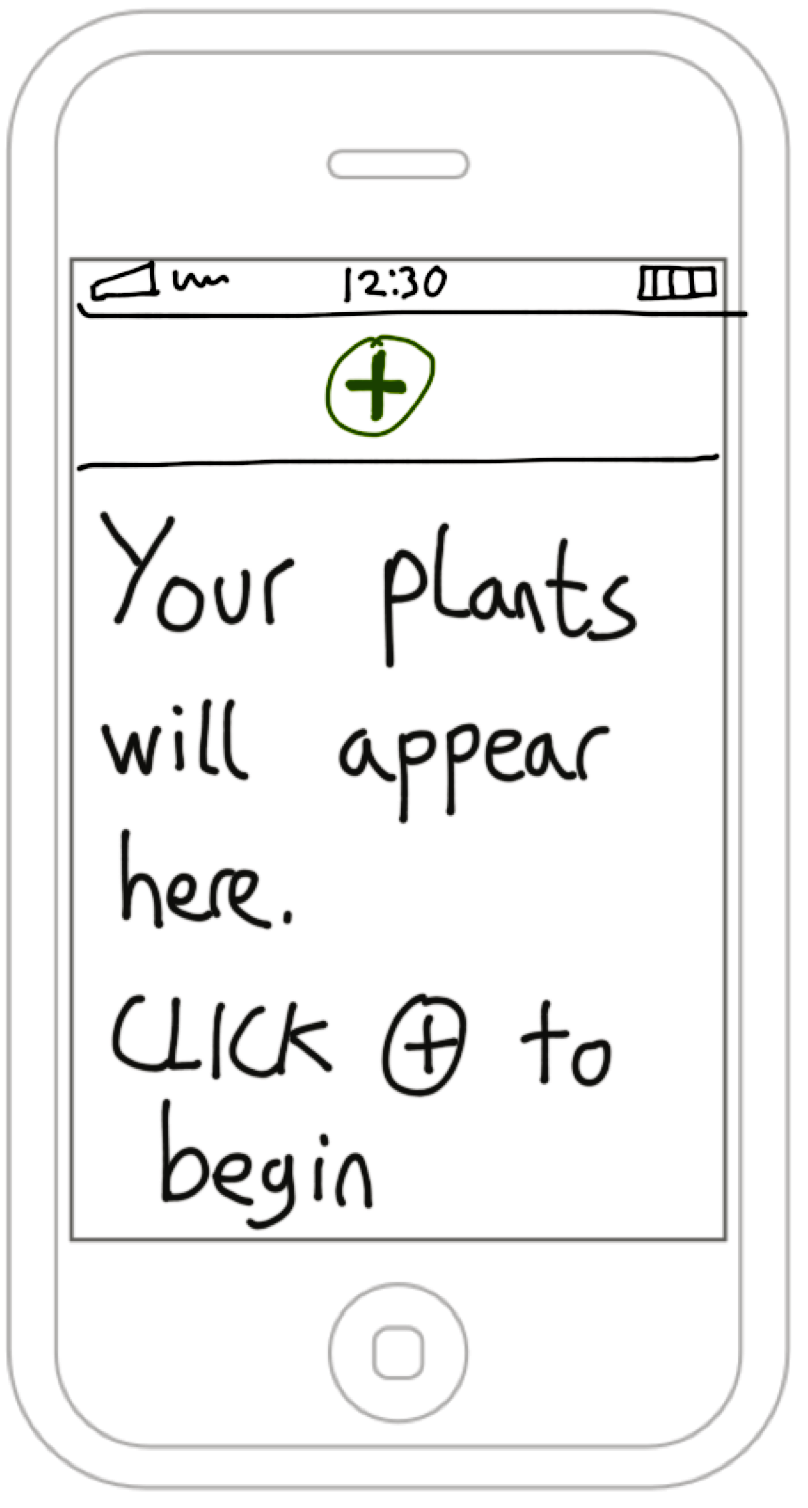
\includegraphics[width=0.22\linewidth]{BeLeaf1.png}
	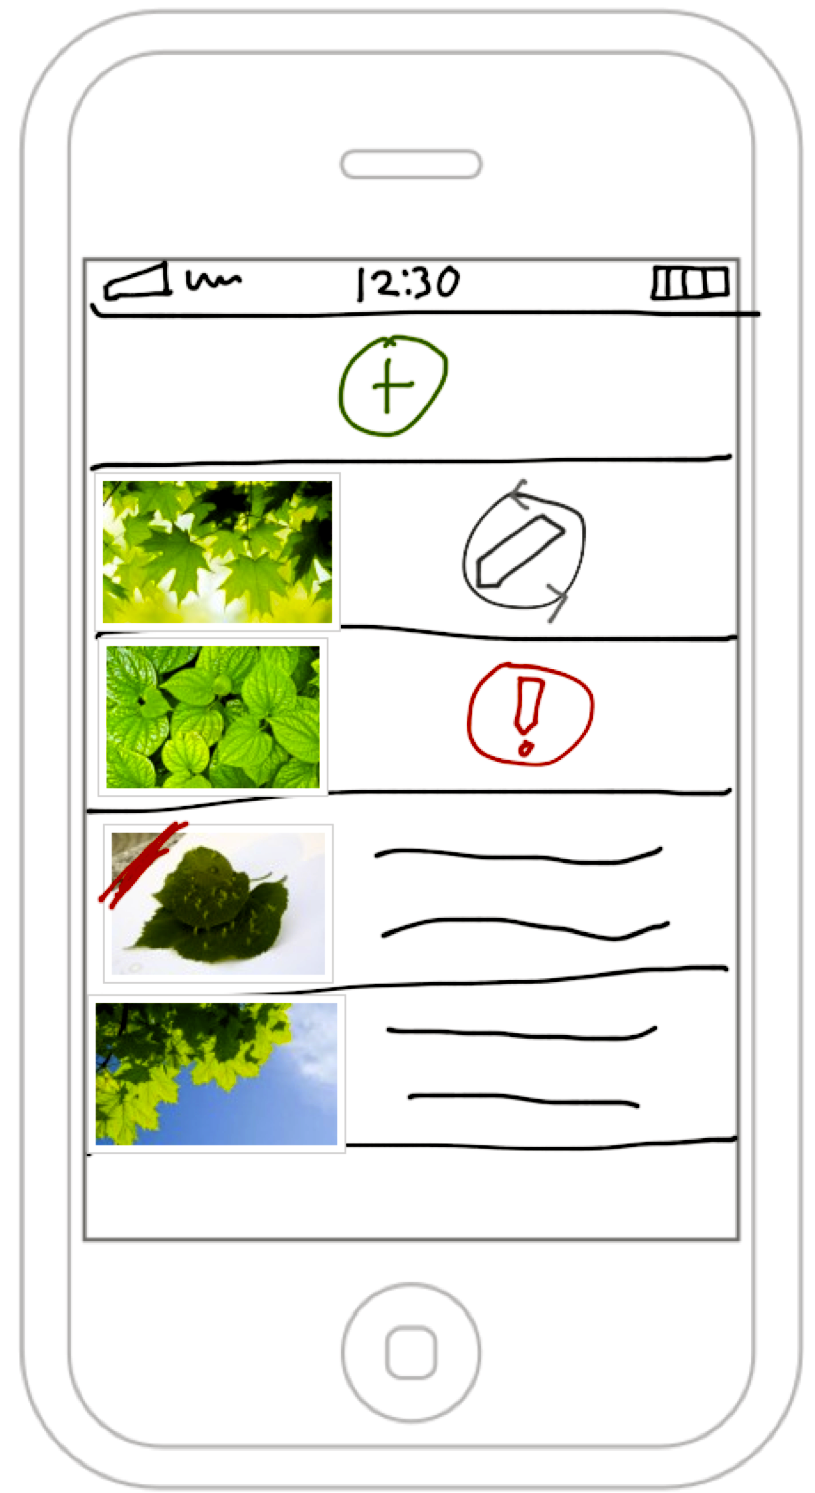
\includegraphics[width=0.19\linewidth]{images/BeLeaf3.png}
	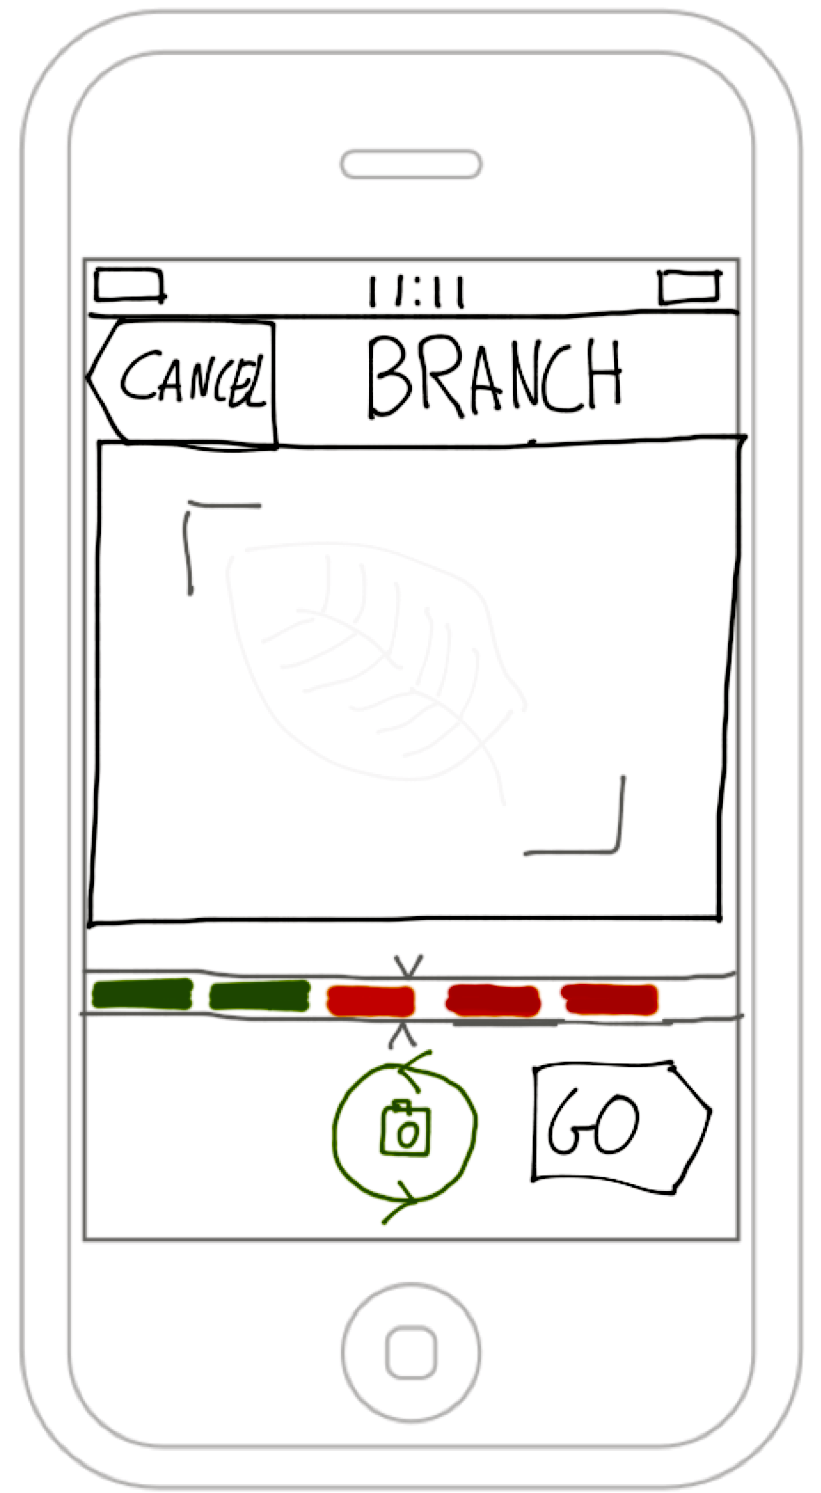
\includegraphics[width=0.19\linewidth]{images/BeLeaf2.png}
	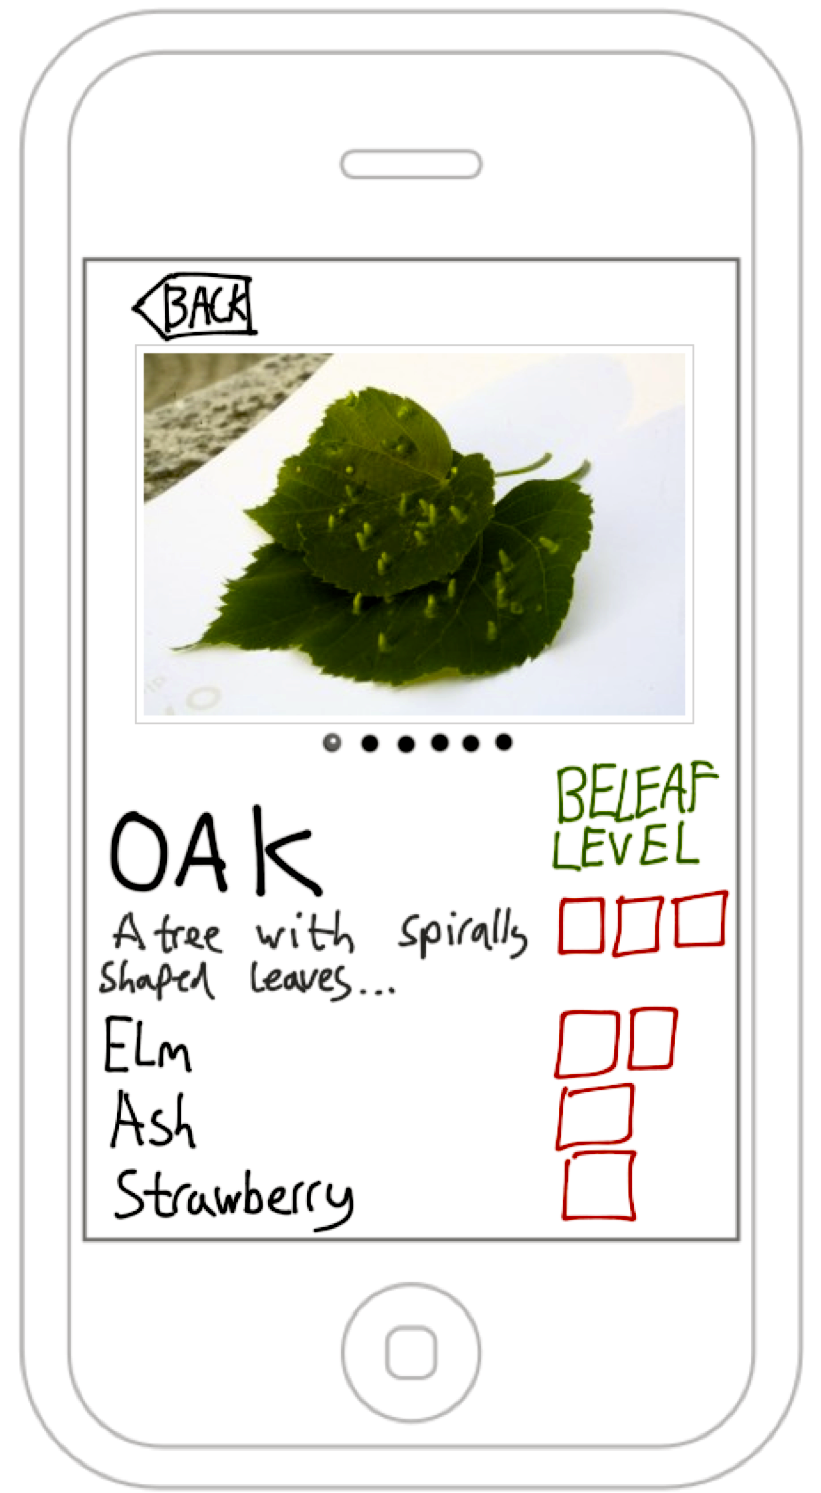
\includegraphics[width=0.19\linewidth]{images/BeLeaf4.png}\\
	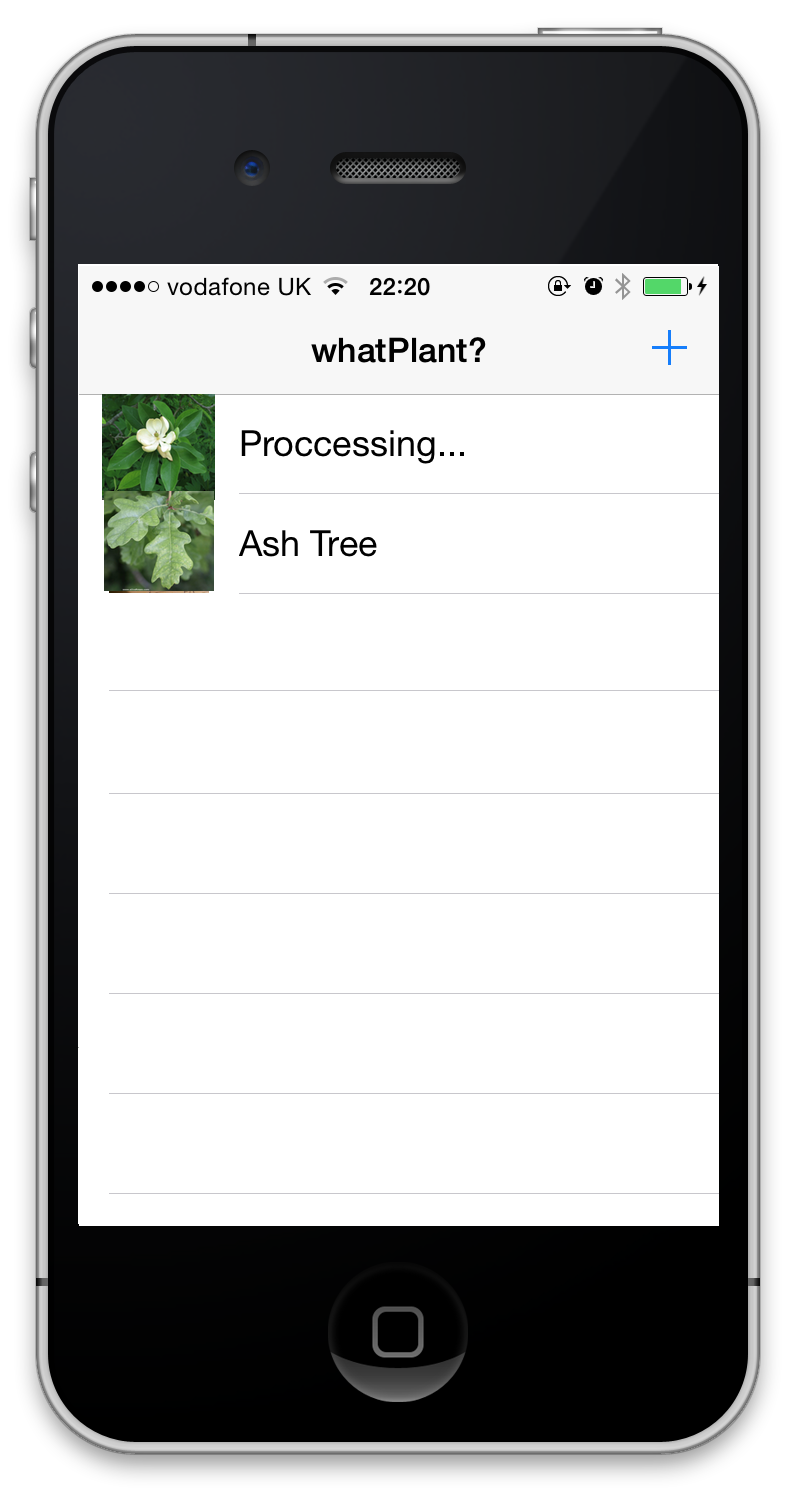
\includegraphics[width=0.19\linewidth]{images/prototypeScreenShot1.png}
	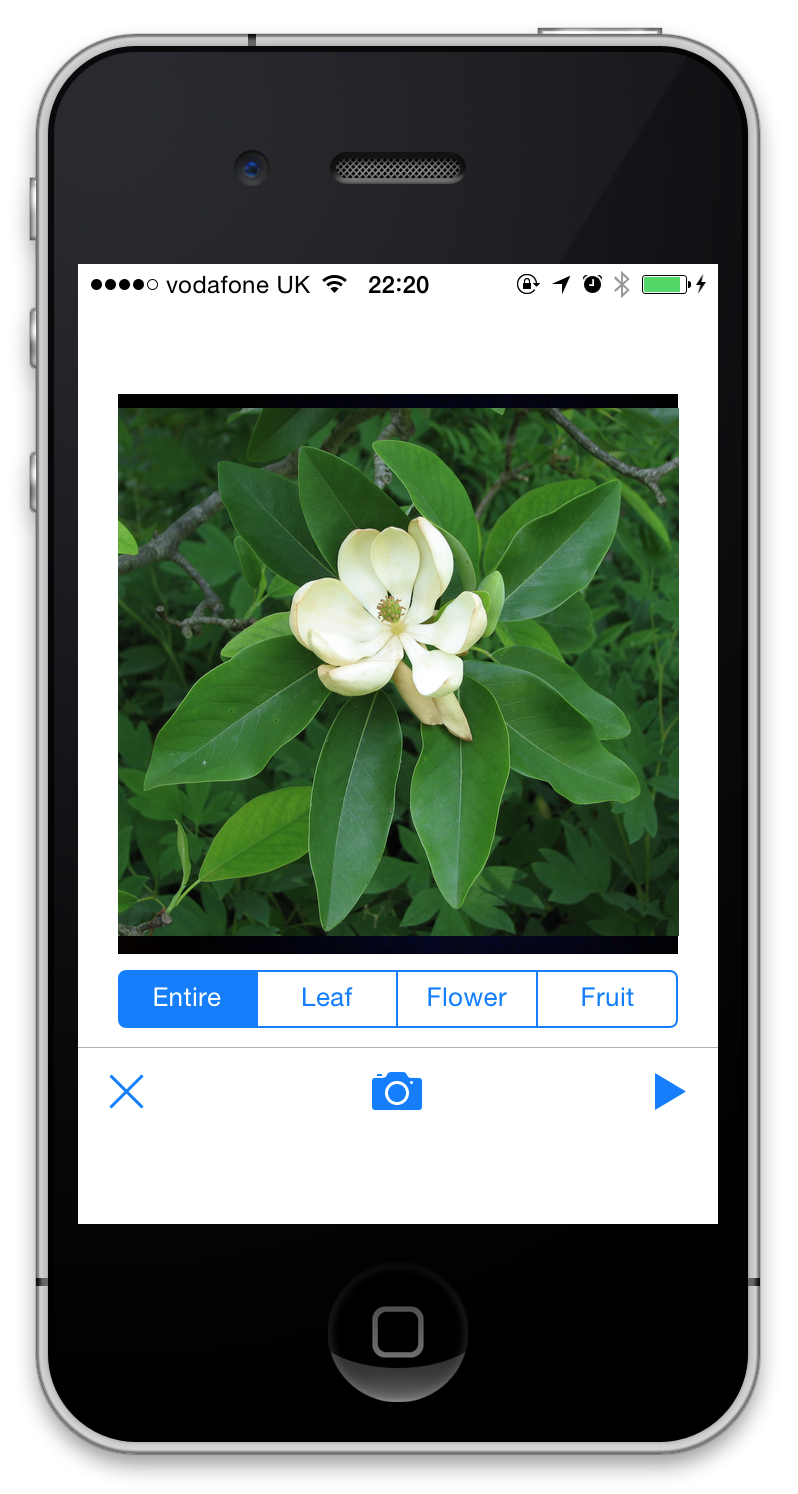
\includegraphics[width=0.19\linewidth]{images/prototypeScreenShot2.png}	
	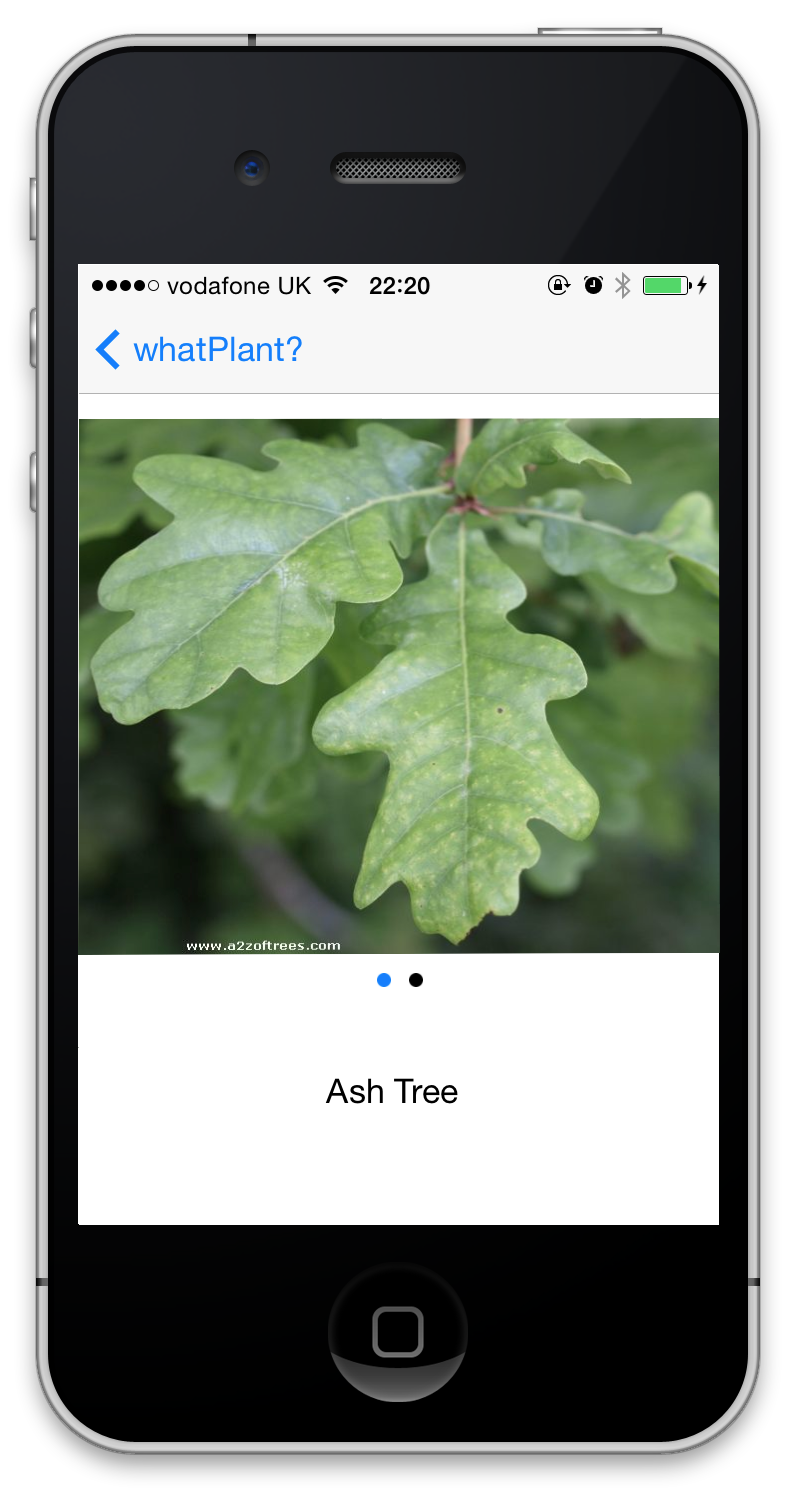
\includegraphics[width=0.19\linewidth]{images/prototypeScreenShot3.png}\\
	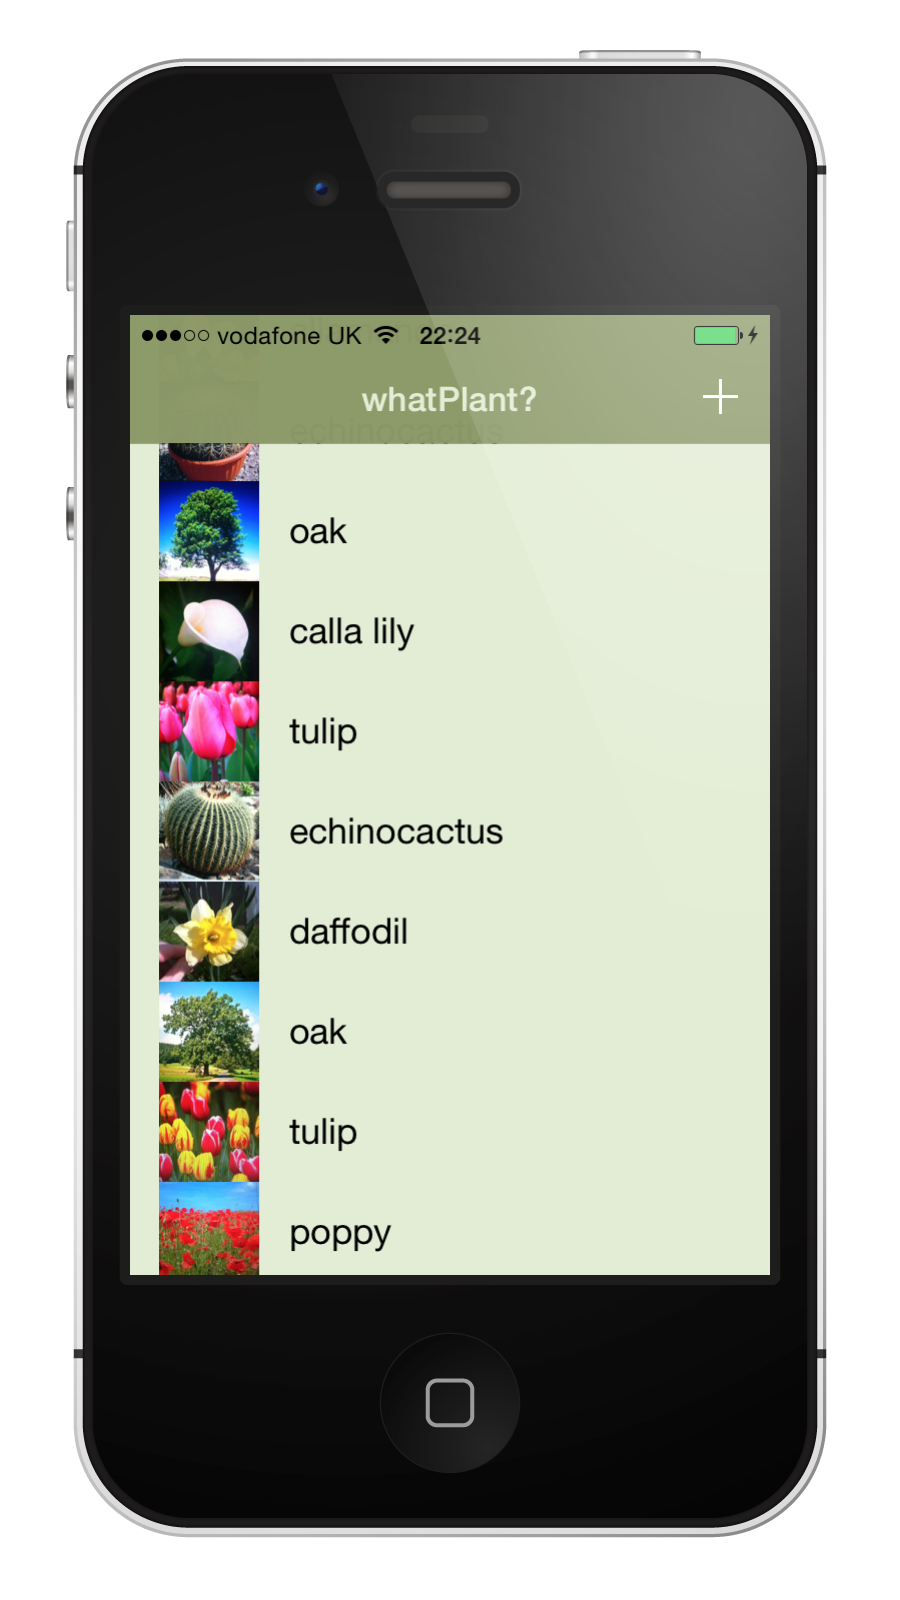
\includegraphics[width=0.22\linewidth]{images/release_1.png}
	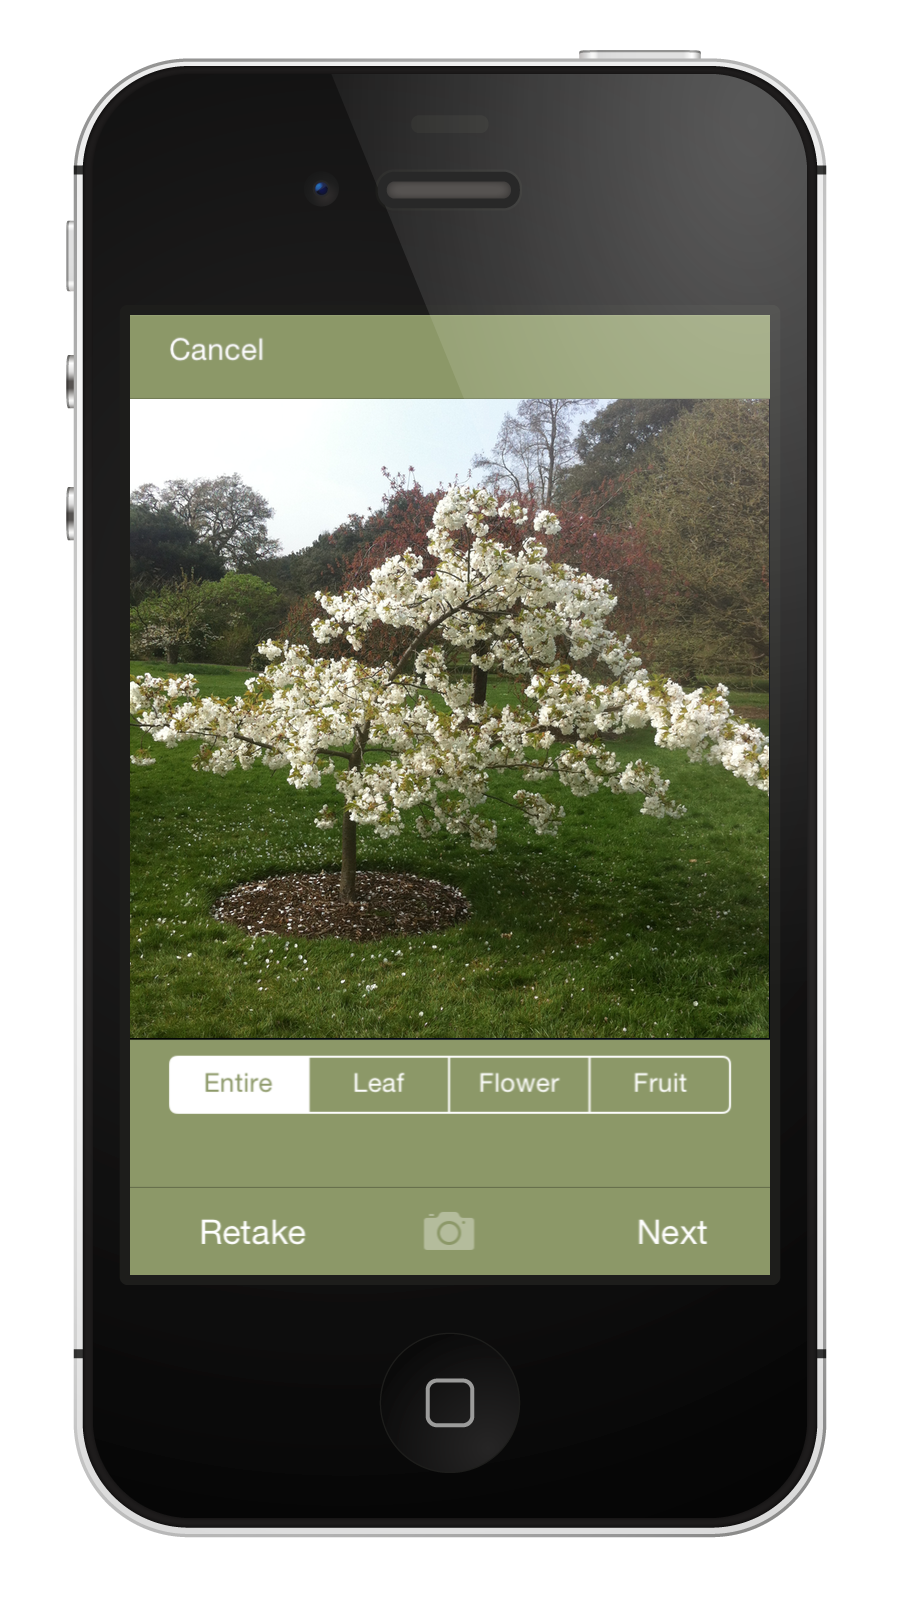
\includegraphics[width=0.22\linewidth]{images/release_2.png}
	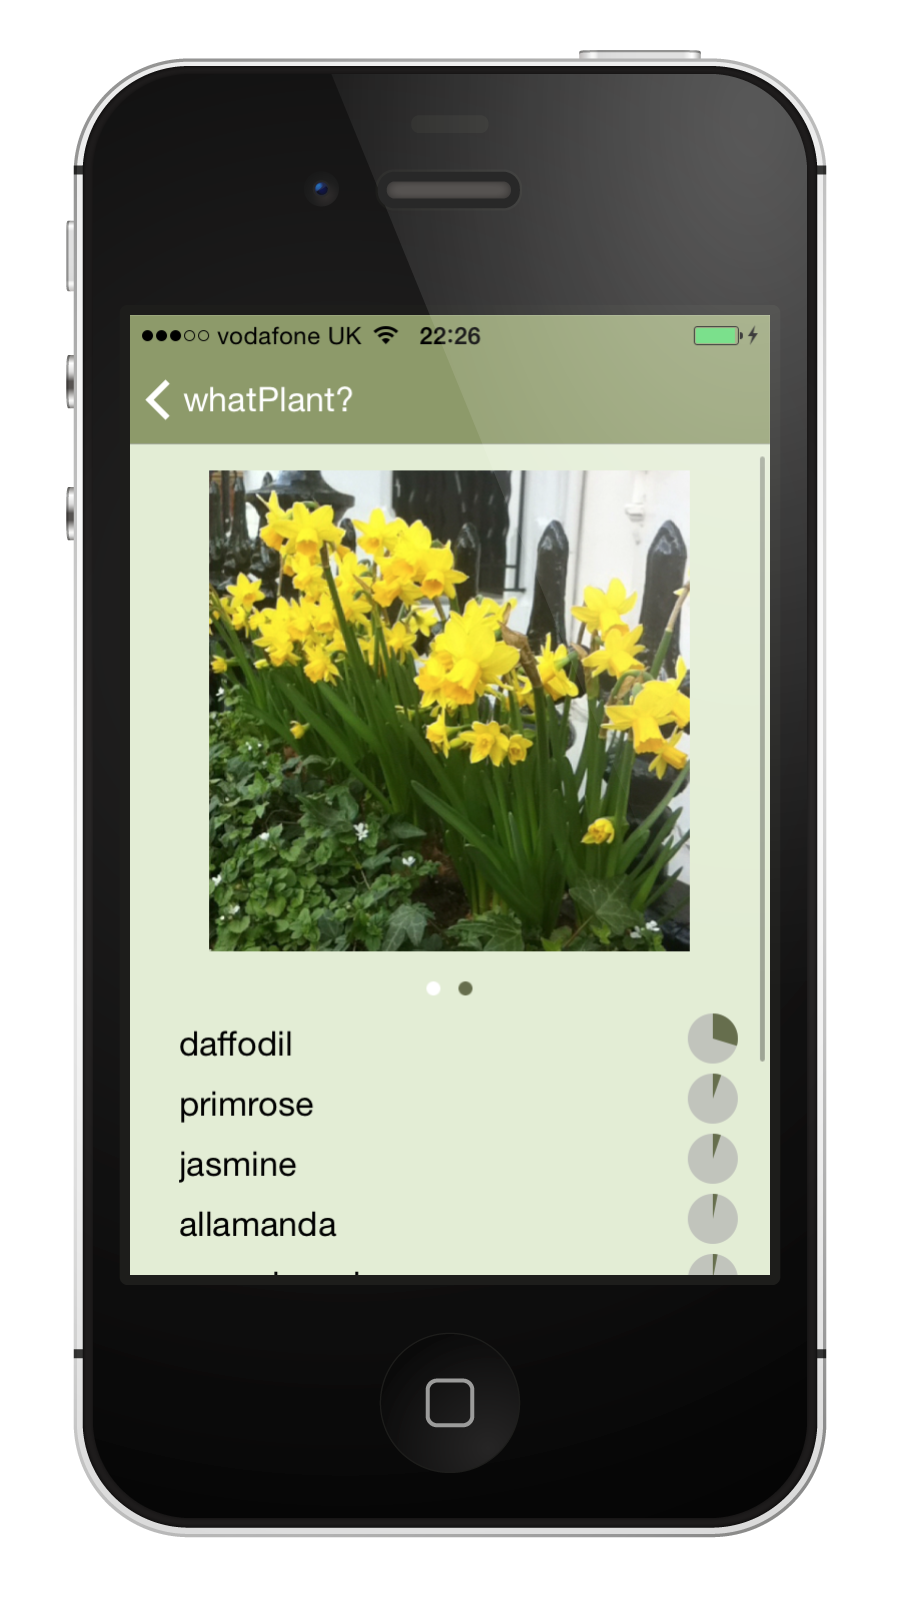
\includegraphics[width=0.22\linewidth]{images/release_3.png}
	\caption{Evolution of the App}
\end{figure}

\begin{figure}[h!]
  \centering
  %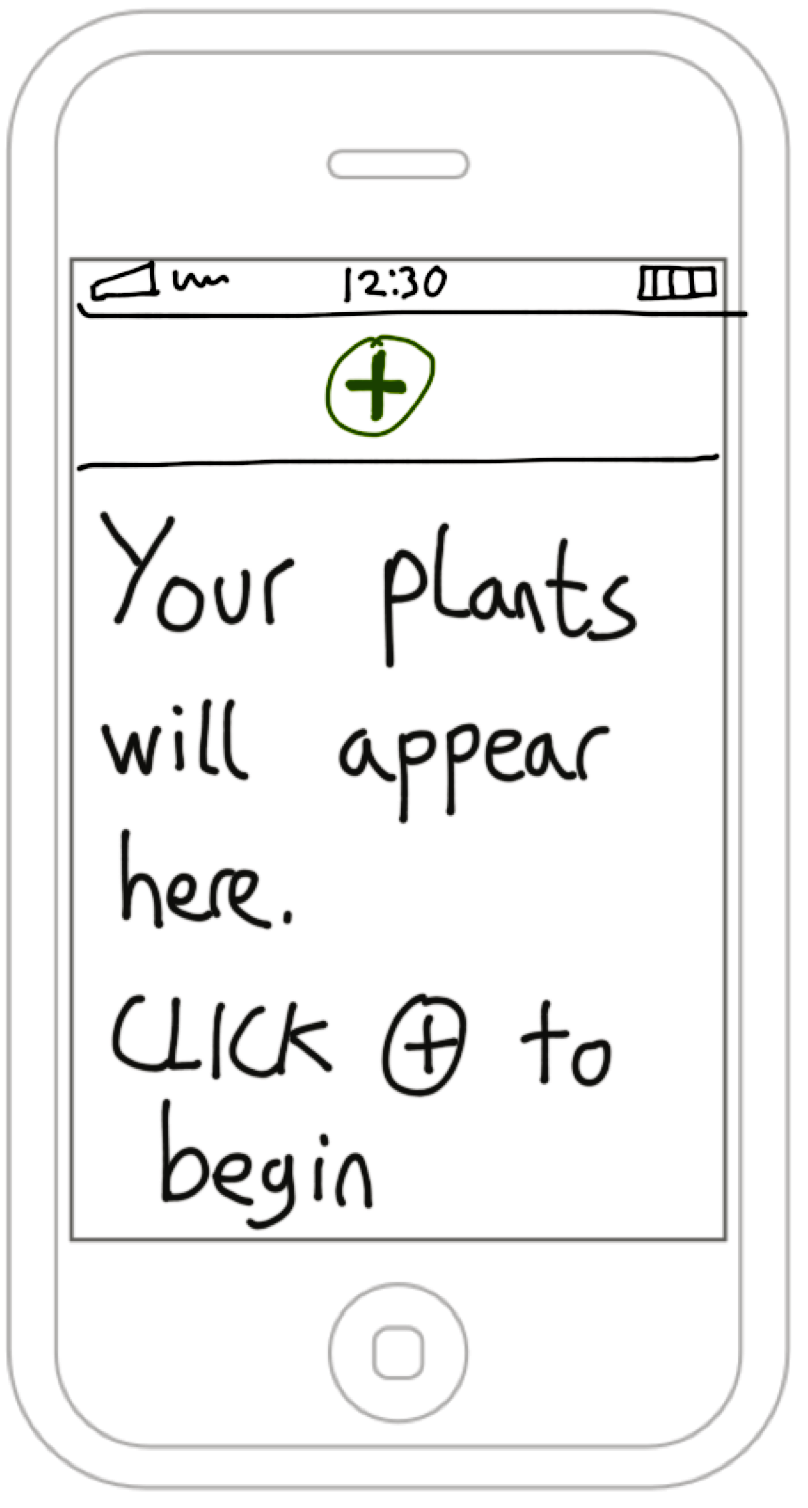
\includegraphics[width=0.22\linewidth]{BeLeaf1.png}
  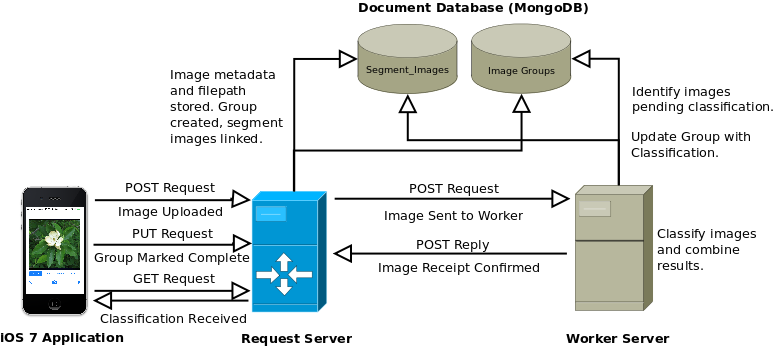
\includegraphics[width=1\linewidth]{SystemContextDiagram.png}
  \caption{System Context Diagram}
  \label{fig:systemcontextdiagram}
\end{figure}

\begin{table}[h]
   \centering
    \begin{tabular}{|l|cc|}
    \hline
    Module                 & Statement Coverage  & Branch Coverage \\ \hline
    Configuration Parsing  & ~   100\% - 52/52   & ~100\% - 22/22     \\
    POST and GET Routes    & ~   81\%  - 102/126   & ~77\%  - 26/34      \\
    Server Instantiation   & ~   88\%  - 46/52   & ~75\%  - 9/12     \\
    \hline
    Total Coverage         &     86\%  - 200/230 & 87\%   - 57/68	\\      
    \hline
    \end{tabular}
    \caption {Code Coverage for Request Server}
\end{table}

\clearpage

\begin{description}

\item [Challenge:] \textit{Data Processing}\\\\
Deep learning itself is distinguished from other machine learning techniques by not simply learning the relative importance of features, but by learning the features themselves. The additional information needed for this raises the desired volume of training data. The PlantCLEF dataset which was originally intended to underlie training, provided a meagre average of 12 images per species; our data sourcing pursuits managed to bring this number up to 2,000 per species. The only significantly large labelled dataset was ImageNet. 

\hspace{5 mm} To ensure our neural network wasn’t burdened having to learn to recognise species for which we had a limited training subset. A Bucketing algorithim was created in order to bucket those images into a higher level in our taxonomy tree which we constructed using WordNet\cite{wordnet}. This meant we could decrease our neural network error rate while maximising our use of available training data. Outlined below is the pseudocode for the bucketing algorithm.\\

\clearpage


\begin{algorithmic}[1]
\Procedure{Update-Descendant-Count}{path}
	\State $count \gets 0$
	\ForAll{$nodes \in path$} 
		\State $count \gets count+NumPlants[node]$
		\State UPDATE Bucket = node, BucketSpecies = Species, Count += count 
		\State		FROM plants 
		\State		WHERE SynsetID = node
	\EndFor
\EndProcedure 
\Statex
\end{algorithmic}

\begin{algorithmic}[1]
\Procedure{Assign-Buckets}{path}
	\For{$i \gets 0 ... path.length$}
		\State $bucket \gets path[i]$
		\State $count \gets NumPlants[bucket]$
		\If{$count >= threshold$}
			\State UPDATE Bucket = $bucket$, BucketSpecies = species 
			\State		FROM plants 
			\State		WHERE SynsetID IN $path[0 ... i]$
			\State break
		\EndIf
	\EndFor
\EndProcedure 
\Statex
\end{algorithmic} 

\end{description}



\appendix
\section{appendix part 1}
\subsection{appendix part 1.1}
\subsection{appendix part 1.2}
\section{appendix part 2}
\subsection{appendix part 2.1}
\subsection{appendix part 2.2}
\end{document}
